\subsection{Sequential Simulation}
% 2 things to show : baseline performance and contrast of dxex v adevs

\subsubsection{Queue}
\label{4-seq-Queue}
% explain what we did: fixed number of models (400, 600 & 800), increasing depth
For the first benchmark, we tested the effect of hierarchical complexity of the model in the performance of the simulator.
A set of three tests was performed, where each test has the same number of models but an increasing depth.
The results can be seen in Figure~\ref{fig:Queue_benchmark_seq}.
Since dxex symbolically flattens the model, there is no performance hit when the depth is increased.
The overhead of running the directconnect algorithm is one time only and negligible when the end time of the simulation is sufficiently large.
Adevs on the other hand does suffer from the increased depth.
With every new hierarchical layer, routing an event from one atomic model to the next becomes more expensive, resulting in an increase in runtime.
\begin{figure}
	\center
	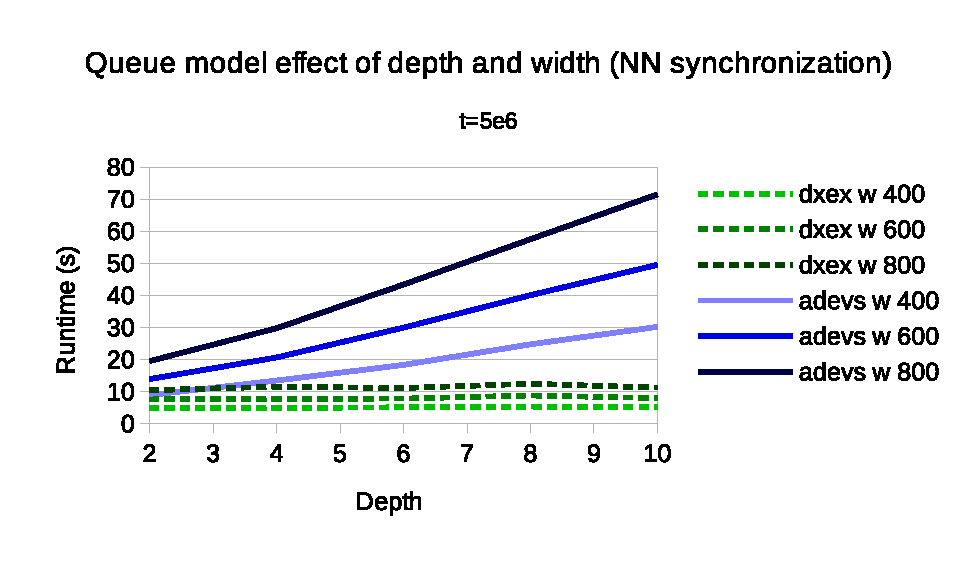
\includegraphics[width=\plotfraction\columnwidth]{fig/queue_fixed_sequential.eps}
	\caption{Queue benchmark results for sequential simulation.}
	\label{fig:Queue_benchmark_seq}
\end{figure}

\subsubsection{Interconnect}
\label{4-seq-Interconnect}
In the Interconnect model, we increase the number of atomic models, thus quadratically increasing the number of couplings and the number of external transitions.
As can be seen in Figure~\ref{fig:Interconnect_benchmark}, adevs outperforms dxex by a fair margin.
Analysis showed that this is caused by the high amount of events: event creation is much slower in dxex than it is in adevs, despite dxex's use of memory pools.
To shield the user from threading and deallocation concerns dxex provides an event superclass from which the user can derive to create a specialized event type.
Copying and deallocation semantics and tracing are solved by the kernels at a runtime cost in simulations where event frequency is very high.
Profiling the benchmarks clearly shows the increasing cost of output generation and deallocation as the determining factor in the gap in performance.
We refer the interested reader to the dxex \hyperref{https://bitbucket.org/bcardoen/devs-ex-machina}{}{repo}{repository} for the profiling call graphs for the different benchmarks.

\begin{figure}
	\center
	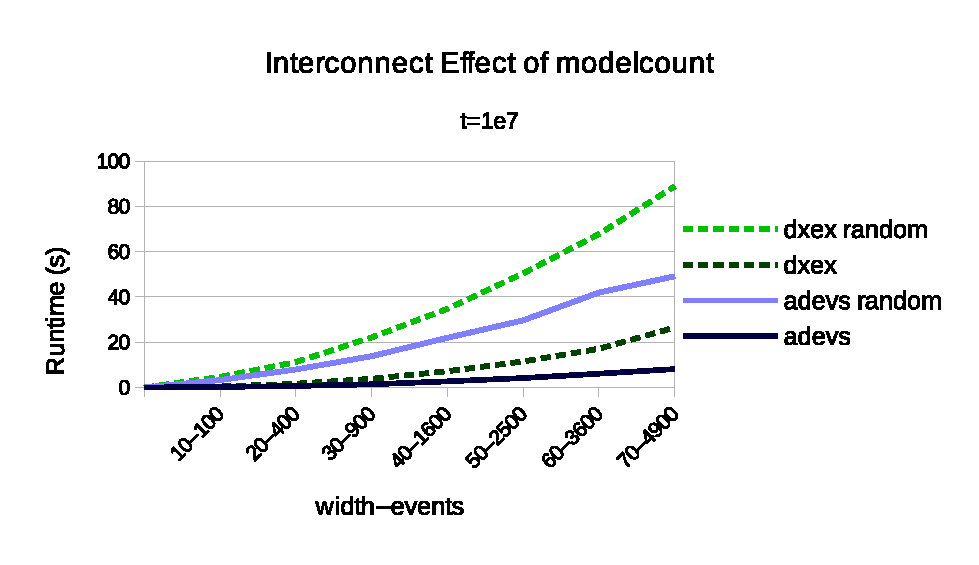
\includegraphics[width=\plotfraction\columnwidth]{fig/interconnect_sequential.eps}
	\caption{Interconnect benchmark results for sequential simulation.}
	\label{fig:Interconnect_benchmark}
\end{figure}

\subsubsection{PHold}
\label{4-seq-PHold}
The PHold model is very similar to the Interconnect model.
The biggest difference is that the amount of messages sent is much lower.
The number of events scales linear with the number of models, not quadratic.
Figure~\ref{fig:Phold_benchmark} shows that the performance of dxex and adevs are very close to each-other, with adevs slightly outperforming dxex.
\begin{figure}
	\center
	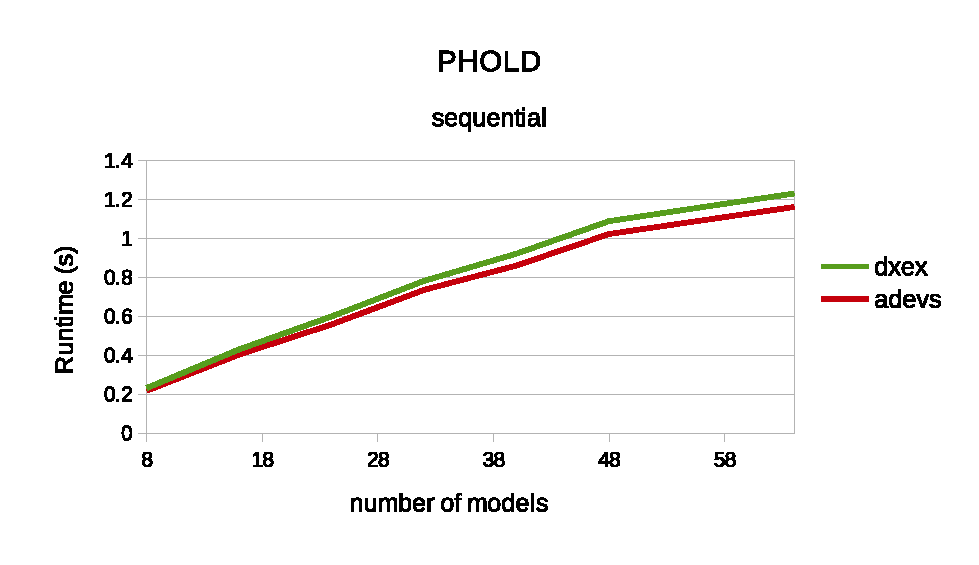
\includegraphics[width=\plotfraction\columnwidth]{fig/phold_sequential.eps}
	\caption{PHold benchmark results for sequential simulation.}
	\label{fig:Phold_benchmark}
\end{figure}
